% FortySecondsCV LaTeX template
% Copyright © 2019-2020 René Wirnata <rene.wirnata@pandascience.net>
% Licensed under the 3-Clause BSD License. See LICENSE file for details.
%
% Please visit https://github.com/PandaScience/FortySecondsCV for the most
% recent version! For bugs or feature requests, please open a new issue on
% github.
%
% Contributors
% ------------
% * ifokkema
% * Bertbk
% * Hespe
%
% Attributions
% ------------
% * fortysecondscv is based on the twentysecondcv class by Carmine Spagnuolo
%   (cspagnuolo@unisa.it), released under the MIT license and available under
%   https://github.com/spagnuolocarmine/TwentySecondsCurriculumVitae-LaTex
% * further attributions are indicated immediately before corresponding code


%-------------------------------------------------------------------------------
%                             ADDITIONAL PACKAGES
%-------------------------------------------------------------------------------

%!TEX program = lualatex
\documentclass[
	a4paper,
	% showframes,
	% vline=2.2em,
	% maincolor=cvgreen,
	% sidecolor=gray!50,
	% sectioncolor=red,
	% subsectioncolor=orange,
	% itemtextcolor=black!80,
	% sidebarwidth=0.4\paperwidth,
	% topbottommargin=0.03\paperheight,
	% leftrightmargin=21pt,
	% rightmarginextra=1cm,
	% profilepicsize=4.5cm,
	% profilepicborderwidth=3.5pt,
	 profilepicstyle=profilecircle,
	% profilepiczoom=1.0,
	% profilepicxshift=0mm,
	% profilepicyshift=0mm,
	% profilepicrounding=1.0cm,
]{fortysecondscv}

% improve word spacing and hyphenation
\usepackage{microtype}
\usepackage{ragged2e}


%  TRYING DIFFERENT FONTS STARTS


% \usepackage[sfdefault]{rosario} % use noto google font

% \usepackage{helvet}
% \renewcommand{\familydefault}{\sfdefault}


% \usepackage[T1]{fontenc}
% \usepackage{Alegreya} %% Option 'black' gives heavier bold face 
% \renewcommand*\oldstylenums[1]{{\AlegreyaOsF #1}}

% \usepackage{fontspec}
% \setmainfont{QTBodini}

% \usepackage{nimbusserif}
% \usepackage[T1]{fontenc}


% \usepackage[sfdefault]{GoSans} % use noto google font
%\usepackage[sfdefault]{noto} % use noto google font



% \usepackage{helvet}
% \renewcommand{\familydefault}{\sfdefault}


% \usepackage{FiraSans}        % Change this to use any font, but keep it simple
% \renewcommand{\familydefault}{\sfdefault}

% \usepackage[sfdefault]{noto} % use noto google font

\usepackage{fontspec}
\setmainfont{Source Sans Pro}[
    BoldFont={Source Sans Pro Bold},
    ItalicFont={Source Sans Pro Italic},
    BoldItalicFont={Source Sans Pro Bold Italic}
]
\newfontfamily{\sourcesansregular}{Source Sans Pro Regular}
\newfontfamily{\sourcesanslight}{Source Sans Pro Light}
\newfontfamily{\sourcesansbold}{Source Sans Pro Bold}
\newfontfamily{\sourcesanssemibold}{Source Sans Pro SemiBold}  % Note: "SemiBold" might need to be one word
\newfontfamily{\merriweather}{Merriweather}[
    BoldFont={Merriweather Bold},
    ItalicFont={Merriweather Italic},
    BoldItalicFont={Merriweather Bold Italic}
]

	% \newfontfamily\headingfont[Path = /Users/ville/Library/Fonts/]{Rosario-VariableFont_wght.ttf} % local font



%  TRYING DIFFERENT FONTS ENDS


% uncomment in case you don't want any hyphenation
\usepackage[none]{hyphenat}




% take care of proper font encoding
\ifxetexorluatex
	\usepackage{fontspec}
	\defaultfontfeatures{Ligatures=TeX}
	%	\newfontfamily\headingfont[Path = fonts/]{segoeuib.ttf} % local font
\else
	\usepackage[utf8]{inputenc}
	\usepackage[T1]{fontenc}
%	\usepackage[sfdefault]{noto} % use noto google font
\fi

% enable mathematical syntax for some symbols like \varnothing
\usepackage{amssymb}

% bubble diagram configuration
\usepackage{smartdiagram}
\smartdiagramset{
	% default font size is \large, so adjust to harmonize with sidebar layout
	bubble center node font = \footnotesize,
	bubble node font = \footnotesize,
	% default: 4cm/2.5cm; make minimum diameter relative to sidebar size
	bubble center node size = 0.4\sidebartextwidth,
	bubble node size = 0.25\sidebartextwidth,
	distance center/other bubbles = 1.5em,
	% set center bubble color
	bubble center node color = maincolor!70,
	% define the list of colors usable in the diagram
	set color list = {maincolor!10, maincolor!40,
	maincolor!20, maincolor!60, maincolor!35},
	% sets the opacity at which the bubbles are shown
	bubble fill opacity = 0.8,
}



%-------------------------------------------------------------------------------
%                            PERSONAL INFORMATION
%-------------------------------------------------------------------------------
%% mandatory information
% your name
\cvname{
    \vspace{3.5cm}
    \begin{center}
        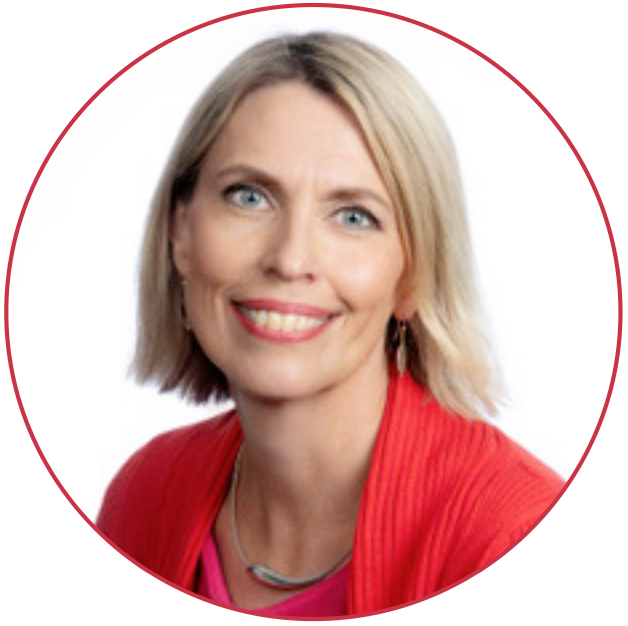
\includegraphics[width=0.6\sidebarwidth]{pics/profile.png}\\[0.5cm]
    \end{center}
    {\merriweather\fontsize{22}{29}\selectfont\textcolor[HTML]{CA3346}{Curriculum Vitae}}\\[-0.3em]
}
% job title/career
\cvjobtitle{}



%-------------------------------------------------------------------------------
%                              SIDEBAR 1st PAGE
%-------------------------------------------------------------------------------
% add more profile sections to sidebar on first page
\addtofrontsidebar{
	% include gosquare national flags from https://github.com/gosquared/flags;
	% naming according to ISO 3166-1 alpha-2 country codes
	\graphicspath{{pics/flags/}}




\aboutme{
    \begin{center}
        \linespread{0.8}
        \selectfont
        {\sourcesansbold\fontsize{8}{13}\selectfont     % Base font size here (11pt with 13pt leading)
        {\sourcesanslight\fontsize{14}{29}\selectfont 1/3}\\[2.5em]
        MD, PhD, Adjunct Professor\\[0.4em]
        Specialist in Gynecology and Obstetrics\\[0.4em]
        Psychotherapist\\[2.2em]
        {\sourcesanslight\fontsize{14}{29}\selectfont KATJA KERO}\\[2em]
        former Langén\\[0.4em]
        Born 5.4.1972 in Turku, Finland\\[0.4em]
        Finnish citizen\\[0.4em]
        Married to specialist\\
        general practioner Markku Kero\\
        Two (adult) children\\[2em]
        {\sourcesansbold\fontsize{9}{11}\selectfont\textcolor[HTML]{CA3346}{LANGUAGE SKILLS}}\\[0.4em]
        Finnish, English, Swedish, (French)\\[2em]
        {\sourcesansbold\fontsize{9}{11}\selectfont\textcolor[HTML]{CA3346}{CONTACT DETAILS}}\\[0.4em]
        Department of Obstetrics\\
        and Gynaecology\\[0.4em]
        Turku University Hospital\\[0.4em]
        Kiinamyllynkatu 4--8\\[0.4em]
        FIN 20520 Turku, Finland\\
        Tel: +358-2-313 0000\\
        Fax: +358-2-313 2340\\[0.4em]
        katja.kero@utu.fi
        }     % End bold font
    \end{center}
}



	
	
}


%-------------------------------------------------------------------------------
%                              SIDEBAR 2nd PAGE
%-------------------------------------------------------------------------------
\addtobacksidebar{



\aboutme{
    \begin{center}
        \linespread{0.8}
        \selectfont
        {\sourcesansbold\fontsize{8}{13}\selectfont     % Base font size here (11pt with 13pt leading)
        {\sourcesanslight\fontsize{14}{29}\selectfont 2/3}\\[2.5em]
        MD, PhD, Adjunct Professor\\[0.4em]
        Specialist in Gynecology and Obstetrics\\[0.4em]
        Psychotherapist\\[2.2em]
        {\sourcesanslight\fontsize{14}{29}\selectfont KATJA KERO}\\[2em]
        }     % End bold font
    \end{center}
}

 
	
}


%-------------------------------------------------------------------------------
%                         TABLE ENTRIES RIGHT COLUMN
%-------------------------------------------------------------------------------
\geometry{right=1cm}  % Adjust the value as needed
\begin{document}


% Change the sidebar and body colors to white
\colorlet{sidecolor}{white}
\colorlet{maincolor}{white}

\makefrontsidebar



% DEFINE MACROS

\newcommand{\HEADER}[1]{
    \cvsection{{\sourcesansbold\fontsize{10.5}{12.5}\selectfont\textcolor[HTML]{CA3346}{#1}}\vspace{-0.5em}}
    \textcolor[HTML]{CA3346}{\hrule}
    \vspace{1em}
}



% For the work experience entries
\newcommand{\TABLESTYLE}[3]{%
    {\sourcesanssemibold\fontsize{8}{10}\selectfont #1} & 
    {\sourcesanslight\fontsize{9.5}{11.5}\selectfont #2}
    {\sourcesanssemibold\fontsize{8}{10}\selectfont\ \ \textcolor[HTML]{CA3346}{•}\ \ #3}\\[0.4em]%
}

\def\SEMIBOLD#1{%
	{\sourcesanssemibold\fontsize{9.5}{10}\selectfont #1\relax}%
}

\def\SEMIBOLDSMALL#1{%
	{\sourcesanssemibold\fontsize{8}{10}\selectfont #1\relax}%
}

\def\SMALLENTER{\\[-0.1em]%
}

\def\ENTER{\\[0.4em]%
}

\def\REGULARSMALL#1{%
	{\sourcesansregular\fontsize{8}{10}\selectfont #1\relax}%
}

\def\REDBALL{%
	\sourcesanssemibold\fontsize{9.5}{11.5}\selectfont \textcolor[HTML]{CA3346}{• }%
}

\def\BALL{%
	\sourcesanssemibold\fontsize{9.5}{11.5}\selectfont{• }%
}


\def\DASH{%
	\sourcesanssemibold\fontsize{9.5}{11.5}\selectfont \textcolor[HTML]{CA3346}{- }%
}

\def\ITALIC#1{%
    {\fontspec{Source Sans Pro Italic} #1\relax}%
}



% DEFINE MACROS ENDS





\HEADER{EDUCATION}
%
\SEMIBOLD{Graduate of Del Oro High School}\SMALLENTER
\SEMIBOLDSMALL{Loomis, California, United States 1990}\ENTER
%
\SEMIBOLD{Matriculation Examination}\SMALLENTER
\SEMIBOLDSMALL{Turun klassillinen Upper Secondary School, Turku, Finland, 1992}\ENTER
%
\SEMIBOLD{Licentiate in Medicine}\SMALLENTER
\SEMIBOLDSMALL{University of Turku, Finland, 2000}\ENTER
%
\SEMIBOLD{Specialist in Gynaecology and Obstetrics}\SMALLENTER
\SEMIBOLDSMALL{University of Turku, Finland, 2009}\ENTER
%
\SEMIBOLD{Basic Sexology Studies (NACS) (30 ECTS)}\SMALLENTER
\SEMIBOLDSMALL{2011}\ENTER
%
\SEMIBOLD{Basic university pedagogy studies (10 ETCS)}\SMALLENTER
\SEMIBOLDSMALL{University of Turku, Finland, 2011--2012}\ENTER
%
\SEMIBOLD{Doctor of Medicine (PhD)}\SMALLENTER
\SEMIBOLDSMALL{University of Turku, Finland, 2014}\ENTER
%
\SEMIBOLD{Psychotherapist in Cognitive Integrative Therapy (65 ECTS)}\SMALLENTER
\SEMIBOLDSMALL{University of Helsinki and Integrum Institute for Cognitive Therapies, Helsinki, Finland, 2021}\ENTER
%
\SEMIBOLD{Cognitive Short Therapy Studies (Year 1, 12 ECTS)}\SMALLENTER
\SEMIBOLDSMALL{Finland, 2020}\ENTER
%
\SEMIBOLD{Specialist in Mindfulness-Based Cognitive Therapies}\SMALLENTER
\SEMIBOLDSMALL{MCBT Program, Finland, 2021}\ENTER
%
\SEMIBOLD{EMDR Therapist}\SMALLENTER
\SEMIBOLDSMALL{EMDR Training Program, Finland, 2022}\ENTER
%
\SEMIBOLD{Special Competence in Medical Education}\SMALLENTER
\SEMIBOLDSMALL{Association of Medical Education in Finland (AMEF), The Finnish Medical Association, 2022}\ENTER
%
\SEMIBOLD{Adjunct Professor (docent)}\SMALLENTER
\SEMIBOLDSMALL{University of Turku, Finland, 2023}\ENTER
%
\SEMIBOLD{Sexual Therapist}\SMALLENTER
\SEMIBOLDSMALL{Sexual Therapy Program, Finland, 2024}





\HEADER{CURRENT POSITIONS}
%
\SEMIBOLD{Physician in charge, Specialist in Obstetrics and Gynaecology}\SMALLENTER
\SEMIBOLDSMALL{Sexual Health Clinic, Turku University Hospital, Finland}\ENTER
%
\SEMIBOLD{Physician in charge, Specialist in Seri Support Centre (TYKS)}\SMALLENTER
\SEMIBOLDSMALL{A care center for victims of sexual assaults}\ENTER
%
{\sourcesanssemibold\fontsize{9.5}{11.5}\selectfont Private practioner in obstetrics and gynaecology and sexological counseling}







\HEADER{CLINICAL EXPERIENCE}
\begin{tabular}{@{}p{0.25\textwidth}p{0.75\textwidth}@{}}
\TABLESTYLE{5/1998-8/1998}{Harjavalta Psychiatric Hospital}{Resident}
%
\TABLESTYLE{5/1999-8/1999}{Health Center of Lavia}{General Practitioner}
%
\TABLESTYLE{5/2000-10/2001}{Health Center of Turku}{General Practitioner}
%
\TABLESTYLE{4/2002-1/2003}{Forssa Hospital}{Resident in Obstetrics and Gynecology}
%
\TABLESTYLE{4/2003-1/2004}{TYKS Loimaa Hospital}{Resident in Obstetrics and Gynecology}
%
\TABLESTYLE{2/2004-7/2006}{Seinäjoki Central Hospital}{Resident in Obstetrics and Gynecology}
%
\TABLESTYLE{9/2006-12/2006}{Turunmaa Hospital}{Resident (Department of Surgery, Urology)}
%
\TABLESTYLE{1/2007-3/2009}{Turku University Hospital}{Resident in Obstetrics and Gynecology}
%
\TABLESTYLE{3/2009-present}{Turku University Hospital}{Specialist in Obstetrics and Gynecology}
%
\TABLESTYLE{7/2009-present}{Self-Employed}{Private Practitioner}
%
\TABLESTYLE{1/2011-12/2021}{Turku University}{Clinical Teacher}
%
\TABLESTYLE{8/2011-present}{Turku University Hospital, Department of Obstetrics and Gynaecology, Sexual Health Clinic}{Physician in Charge, Specialist}
%
{\sourcesanssemibold\fontsize{8}{10}\selectfont 5/2019-present} & {\sourcesanslight\fontsize{9.5}{11.5}\selectfont Turku University Hospital, Seri Support Centre}\\[-0.1em]
\phantom{XXXXX} & {\sourcesanssemibold\fontsize{8}{10}\selectfont \textcolor[HTML]{CA3346}{•}\ \ Physician in Charge, Specialist}
\end{tabular}



% \vspace{1em} % Adds a single empty line

 

 
\newpage

\begin{sidebar}
    \begin{center}
        \linespread{0.8}
        \selectfont
        \vspace{32em}
        {\merriweather\fontsize{22}{29}\selectfont\textcolor[HTML]{CA3346}{Curriculum}}\\[1.1em]
		{\merriweather\fontsize{22}{29}\selectfont\textcolor[HTML]{CA3346}{Vitae}}\\[2em]
        {\sourcesansbold\fontsize{8}{13}\selectfont     % Base font size here (11pt with 13pt leading)
        {\sourcesanslight\fontsize{14}{29}\selectfont 2/3}\\[2.5em]
        MD, PhD, Adjunct Professor\\[0.4em]
        Specialist in Gynecology and Obstetrics\\[0.4em]
        Psychotherapist\\[2.2em]
        {\sourcesanslight\fontsize{14}{29}\selectfont KATJA KERO}\\[2em]
        }
    \end{center}
\end{sidebar}

% \newgeometry{
% 	top=\topbottommargin,
% 	bottom=\topbottommargin,
% 	right=\leftrightmargin,
% 	left=\leftrightmargin
% }


 
\HEADER{ACTIVITIES IN THE ACADEMIC COMMUNITY}

\SEMIBOLD{Mannerheim League for Child Welfare, Littoinen}\SMALLENTER
\SEMIBOLDSMALL{Member of the Board 2008–2012}\ENTER
%
\SEMIBOLD{The Finnish Gynecological Association}\SMALLENTER
\SEMIBOLDSMALL{Secretary 2016–2017}\ENTER
%
\SEMIBOLD{The Committee for the Promotion of Sexual and Reproductive Health in Finland Proper}\SMALLENTER
\SEMIBOLDSMALL{Chairman 2020–2021}\ENTER
\SEMIBOLDSMALL{Vice-Chairman 2016–2019}\ENTER
\SEMIBOLDSMALL{Member of the Board 2015–2019}\ENTER
%
\SEMIBOLD{The Sexual Health Group of the Finnish Gynecological Association}\SMALLENTER
\SEMIBOLDSMALL{Chairman 2018–present}\ENTER
%
\SEMIBOLD{The Finnish Gynecological Association's Sexual Health Group}\SMALLENTER
\SEMIBOLDSMALL{Member of the Board 2010–present}\ENTER
%
\SEMIBOLD{The Finnish Gynecological Association's Sexual Health Group}\SMALLENTER
\SEMIBOLDSMALL{Member of the Board 2018–2022}\ENTER
%
\SEMIBOLD{The Nordic Society of Sexual Medicine}\SMALLENTER
\SEMIBOLDSMALL{Member of the Board 2022–present}\ENTER
\SEMIBOLDSMALL{Vice President 2023–present}\ENTER
\SEMIBOLDSMALL{President 2024–present}\ENTER
%
\SEMIBOLD{The HPV Coalition}\SMALLENTER
\SEMIBOLDSMALL{Member;}
\REGULARSMALL{The coalition is founded by experts and a patient organization, whose goal is to promote Finland's commitment to the EU's cancer control plan's goal of eradicating cancers caused by HPV.}\ENTER
%
\SEMIBOLD{The Korento ry}\SMALLENTER
\SEMIBOLDSMALL{Expert member / "godmother";}
\REGULARSMALL{Korento ry is a national patient organization that represents up to 200,000 Finns living with endometriosis, adenomyosis, PCOS, and vulvodynia.}\ENTER
%
\SEMIBOLD{The Gynecological Cancer Patients Association of Finland}\SMALLENTER
%
\SEMIBOLDSMALL{Expert member}










\HEADER{RESEARCH GRANTS}

\SEMIBOLD{The Cancer Foundations of South-Western Finland, 4,000 €}\ENTER
%
\SEMIBOLD{The Cancer Foundations of Finland, 3,400 €}\ENTER
%
\SEMIBOLD{The Finnish Gynaecological Society, 4,000 €}\ENTER
%
\SEMIBOLD{The Finnish Medical Foundation, 2,500 €}\ENTER
%
\SEMIBOLD{The Finnish Medical Foundation, 4,000 €}\ENTER
%
\SEMIBOLD{The Finnish Society Against Sexually Transmitted Diseases, 3,000 €}\ENTER
%
\SEMIBOLD{National Graduate School of Clinical Investigation, 3,500 €}\ENTER
%
\SEMIBOLD{The Government Special Foundation (EVO) to Turku University Hospital, 14,000 €}\ENTER
%
\SEMIBOLD{Orion-Pharmos Research Foundation, 3,000 €}\ENTER
\SEMIBOLD{Project on implementation of education of sexual medicine  in Finnish medical schools}\SMALLENTER
\phantom{XXX}\SEMIBOLD{\BALL The Finnish Medical Foundation:}\\
\phantom{XXX}{- 3,000 € {\SEMIBOLDSMALL{for the study of developing education of Sexual Medicine for Medical Schools (2019)}}\\
\phantom{XXX}{- 3,500 € {\SEMIBOLDSMALL{for the study of developing education of Sexual Medicine for Medical Schools (2021,}}\\
\phantom{XXXX}{\SEMIBOLDSMALL{producing lectures and other materials for the Medical Schools of Finland)}}\ENTER
%
\SEMIBOLD{Project focusing on vaginal and oral microbiota ("EMMI")}\SMALLENTER
\phantom{XXX}{\BALL The Cancer Foundations of South-Western Finland: 8,500 € {\sourcesanssemibold\fontsize{8}{10}\selectfont (12/2016)}}\\
\phantom{XXX}{\BALL The Government Special Foundation (EVO) to Turku}\SMALLENTER
\phantom{XXXX}{\SEMIBOLD{University Hospital: 5,000 €} {\sourcesanssemibold\fontsize{8}{10}\selectfont (12/2016)}}\\
\phantom{XXX}{\BALL The Finnish Cultural Foundation: 24,000 € {\sourcesanssemibold\fontsize{8}{10}\selectfont for DNA analyses (5/2020)}}\ENTER
%
\SEMIBOLD{Project focusing on eradicating domestic violence (EHYEKSI-hanke)}\SMALLENTER
\phantom{XXX}\SEMIBOLD{\BALL Päivikki and Sakari Sohlberg Foundation: 15,000 €}\\






\newpage

\begin{sidebar}
    \begin{center}
        \linespread{0.8}
        \selectfont
        \vspace{32em}
        {\merriweather\fontsize{22}{29}\selectfont\textcolor[HTML]{CA3346}{Curriculum}}\\[1.1em]
		{\merriweather\fontsize{22}{29}\selectfont\textcolor[HTML]{CA3346}{Vitae}}\\[2em]
        {\sourcesansbold\fontsize{8}{13}\selectfont     % Base font size here (11pt with 13pt leading)
        {\sourcesanslight\fontsize{14}{29}\selectfont 2/3}\\[2.5em]
        MD, PhD, Adjunct Professor\\[0.4em]
        Specialist in Gynecology and Obstetrics\\[0.4em]
        Psychotherapist\\[2.2em]
        {\sourcesanslight\fontsize{14}{29}\selectfont KATJA KERO}\\[2em]
        }
    \end{center}
\end{sidebar}


% \newgeometry{
% 	top=\topbottommargin,
% 	bottom=\topbottommargin,
% 	right=\leftrightmargin,
% 	left=\leftrightmargin
% }


 

 




\HEADER{HONOURS AND PRIZES}

\SEMIBOLD{Recipient of the Best Thesis Award in 2014}\SMALLENTER
\SEMIBOLDSMALL{The Finnish Gynaecological Society, Ulla-Maija Mäkilä Fund}\ENTER
%
\SEMIBOLD{Recipient of the Best Thesis Award in 2014}\SMALLENTER
\SEMIBOLDSMALL{Turunmaa Duodecim Medical Society}






 





\HEADER{PHD THESES UNDER SUPERVISION}


{\SEMIBOLD{TtM Sanna-Mari Manninen:}\ITALIC{"Sexual Education in Finland: A National Survey among Medical Students and General Practitioners"}}\\[-0.1em]
\phantom{X}\SEMIBOLDSMALL{• Completed her PhD on 8.5.2024 at the University of Turku}\ENTER
{\sourcesanssemibold\fontsize{9.5}{11.5}\selectfont LL Anna Aromaa's Dissertation: }\ITALIC{"Do Gynecologists Talk about Sexual Health? Attitudes,\linebreak Perceived Barriers, Practice Patterns and Education of Sexual Medicine in Finland: A National Survey among Gynecologists and Obstetricians"}\\[-0.1em]
%
\phantom{X}\SEMIBOLDSMALL{• The first partial publication published}\SMALLENTER
\phantom{X}\SEMIBOLDSMALL{• The second publication submitted to an international peer-reviewed journal}\ENTER
%
{\sourcesanssemibold\fontsize{9.5}{11.5}\selectfont LK Viivi Virkkunen's Doctoral Thesis: }\ITALIC{"The connection of vascular health, physical activity and fitness to women's sexual function in women of retirement age and the effect of retirement on women's sexual function"}\\[-0.1em]
\phantom{X}\SEMIBOLDSMALL{• First partial publication published in a peer-reviewed journal}\SMALLENTER
\phantom{X}\SEMIBOLDSMALL{• The second publication submitted}






\HEADER{PUBLICATIONS}

\SEMIBOLD{Total: 53}\ENTER
%
\phantom{}\SEMIBOLD{Original publications: 22 in international academic journals (total IF count: 163.37), 2 in Finnish journals}\ENTER
%
\phantom{}\SEMIBOLD{Review articles and book chapters: 23}\ENTER
%
\phantom{}\SEMIBOLD{Editorials: 6}\ENTER
%
\phantom{}\SEMIBOLD{Submitted publications: 3 original articles}\ENTER
%
\phantom{}\SEMIBOLD{Poster presentations: 9}\ENTER
%
\phantom{}\SEMIBOLD{Total sum of citations: 201}\ENTER
%
\phantom{}\SEMIBOLD{Web of Science h-index: 8}








\HEADER{WORK AS AN EDITOR}
%
\SEMIBOLD{Ambitious work as one of the four editors of the first Finnish-language
 book on Sexual Medicine (761 pages, 42 authors) published by Duodecim Publishing
 Company Ltd 2020. The first edition is almost sold out and the second edition is
 currently being worked on. In addition to editing, I have written 9 chapters in the
 book. Editing the book included reviewing chapters and helping other authors
 writing their texts.}\ENTER
\SEMIBOLDSMALL{https://www.duodecim.fi/english/}\ENTER
%
\SEMIBOLD{Editor of the special theme number "Impact of disease on sexual health"
 of the Academic Journal Duodecim with Professor Päivi Polo. Also wrote one
 article and an Editorial for this issue.}\ENTER
\SEMIBOLDSMALL{https://www.duodecim.fi/2021/10/20/duodecim-lehti-nro-20-on-ilmestynyt-teemana-krooninen-sairaus-}\SMALLENTER
\SEMIBOLDSMALL{ja-seksuaalisuus/}\ENTER
%
\SEMIBOLD{Numerous scientific and other presentations internationally and nationally.}









\HEADER{CLINICAL VISITS ABROAD}

\SEMIBOLD{As a medical student: Budapest, Hungary 1998}\ENTER
%
\SEMIBOLD{As a clinical teacher with medical students: Dublin, Ireland 2012; Madrid, Spain 2013; Nice, France 2014; Amsterdam, The Netherlands 2016; Lisbon, Portugal 2017}\ENTER
%
\SEMIBOLD{A visit to a sexological clinic: Aalborg, Denmark 2018}
\phantom{}\SEMIBOLD{Aalborg, Denmark 2018}





\end{document}

